

\begin{question}
	\questiontext{Balance, weak balance and unbalanced networks}
	All of the implementations for this question are provided inside the q4.ipynb file
	\begin{subquestion}{Sign prediction}
		\answer{
			Our algorithm uses a backtracking search to determine if a graph can be "balanced" by assigning positive ($+1$) or negative ($-1$) signs to a specific set of unassigned edges (zero\_edges). It operates by recursively iterating through each unassigned edge and tentatively assigning it a sign, immediately checking if that choice violates the "balance" condition of any associated triangles (triangle\_edges). a triangle is considered balanced if the product of its edge signs is positive (i.e., it contains an even number of negative edges). By performing this "pruning" check early—ensuring a triangle is still valid as soon as an edge within it is signed—the algorithm avoids exploring invalid branches of the search tree. If the algorithm successfully assigns signs to all edges such that every triangle in the set satisfies the balance condition, it returns True; otherwise, it backtracks, resets the edge, and tries a different configuration, returning False if no valid assignment exists.
		}
	\end{subquestion}
	
	\begin{subquestion}{Balance test:}
		\answer{
		Our algorithm evaluates structural balance in a signed graph by identifying "factions" (super-nodes) and analyzing the relationships between them. It begins by isolating all positive edges to determine the graph’s connected components, which represent groups of "friends" that should ideally belong to the same cluster. If any negative edge exists within one of these clusters, it immediately flags a structural contradiction and labels the graph as unbalanced. If internal clusters are consistent, the algorithm constructs a "reduced graph" where each cluster is treated as a single node, connected by the original negative edges. A graph is then declared strongly balanced if this reduced graph is bipartite—meaning all nodes can be split into two opposing camps with no internal conflict—or weakly balanced if there are no internal negative edges but more than two camps exist. Finally, the draw\_clusters function generates a visual map, color-coding nodes by their cluster membership and edges by their sign (blue for positive, red for negative) using a Fruchterman-Reingold layout to reveal the social structure.
	}
	\newpage
\answer{
		\textbf{Network A}
		\textbf{Identified Super-nodes:} 3 factions\\
		\textbf{Result:} Strongly balanced\\
		\textbf{Reason:} The reduced graph is bipartite.
		
		\paragraph{Super-node Assignments}
		\begin{itemize}
			\item Super-node 0 (Size 28): $\{0,2,4,6,9,27,29,1,22,26,15,31,32 \\\hfill
			,33,34,3,7,8,19,24,12,20,5,16,25,11,30,13\}$
			\item Super-node 1 (Size 4): $\{10,14,21,23\}$
			\item Super-node 2 (Size 3): $\{17,18,28\}$
		\end{itemize}
	}
		\begin{figure}[H]
			\centering
			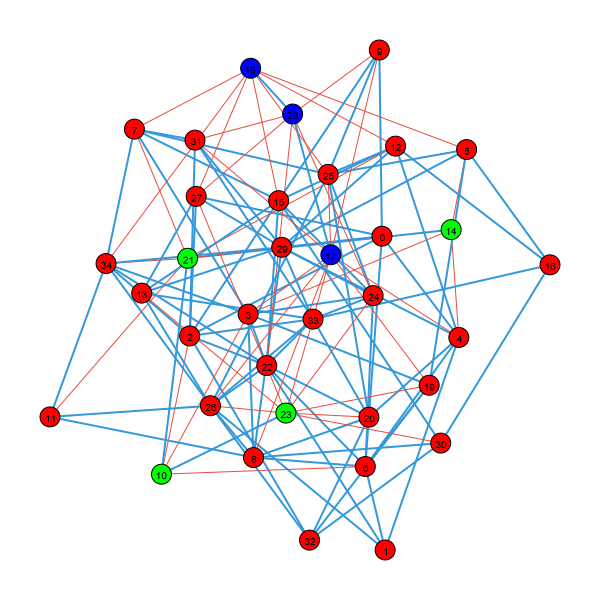
\includegraphics[width=0.6\textwidth]{imgs/clusters_network_a.png}
			\caption{Colored  graph of Network A by supernode assignments}
		\end{figure}
		\newpage
	\answer{
		\textbf{Network B}
		\textbf{Identified Super-nodes:} 3 factions\\
		\textbf{Result:} Unbalanced\\
		\textbf{Reason:} Internal contradiction: nodes 0 and 14 belong to the same super-node but are connected by a negative edge.
		
		\paragraph{Super-node Assignments}
		\begin{itemize}
			\item Super-node 0 (Size 36): $\{0,3,7,9,11,14,21,28,30,34,35,36,1,13,19,32,2\\\hfill
			,5,24,20,26,27,29,31,4,37,18,10,25,33,8,12,17,23,16,22\}$
			\item Super-node 1 (Size 1): $\{6\}$
			\item Super-node 2 (Size 1): $\{15\}$
		\end{itemize}
	}
		\begin{figure}[H]
			\centering
			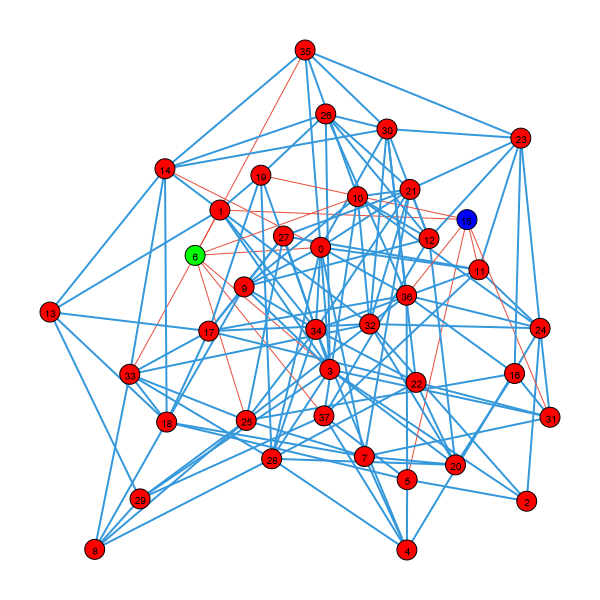
\includegraphics[width=0.6\textwidth]{imgs/clusters_network_b.png}
			\caption{Colored  graph of Network B by supernode assignments}
		\end{figure}
		\newpage
		\answer{
		\textbf{Network C}
		\textbf{Identified Super-nodes:} 3 factions\\
		\textbf{Result:} Unbalanced\\
		\textbf{Reason:} The reduced graph contains an odd cycle.
		
		\paragraph{Super-node Assignments}
		\begin{itemize}
			\item Super-node 0 (Size 15): $\{0,8,9,11,28,31,6,7,21,25,27,4,16,29,30\}$
			\item Super-node 1 (Size 19): $\{23,1,2,3,10,20,22,32,34,18,19,24,5,12,17,26,13,14,15\}$
			\item Super-node 2 (Size 1): $\{33\}$
		\end{itemize}
	}
		\begin{figure}[H]
			\centering
			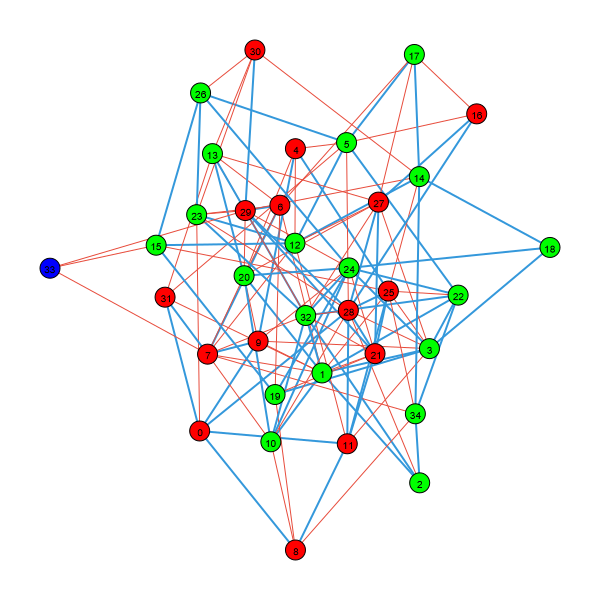
\includegraphics[width=0.6\textwidth]{imgs/clusters_network_c.png}
			\caption{Colored  graph of Network C by supernode assignments}
		\end{figure}
		\newpage
		\answer{
		\textbf{Network D}
		\textbf{Identified Super-nodes:} 5 factions\\
		\textbf{Result:} Unbalanced\\
		\textbf{Reason:} Internal contradiction: nodes 3 and 13 are grouped together but share a negative edge.
		
		\paragraph{Super-node Assignments}
		\begin{itemize}
			\item Super-node 0 (Size 17): $\{0,1,10,11,25,12,15,17,26,7,8,21,16,20,27,18,23\}$
			\item Super-node 1 (Size 1): $\{6\}$
			\item Super-node 2 (Size 1): $\{24\}$
			\item Super-node 3 (Size 1): $\{2\}$
			\item Super-node 4 (Size 9): $\{9,14,28,3,13,19,4,22,5\}$
		\end{itemize}
	}
		\begin{figure}[H]
			\centering
			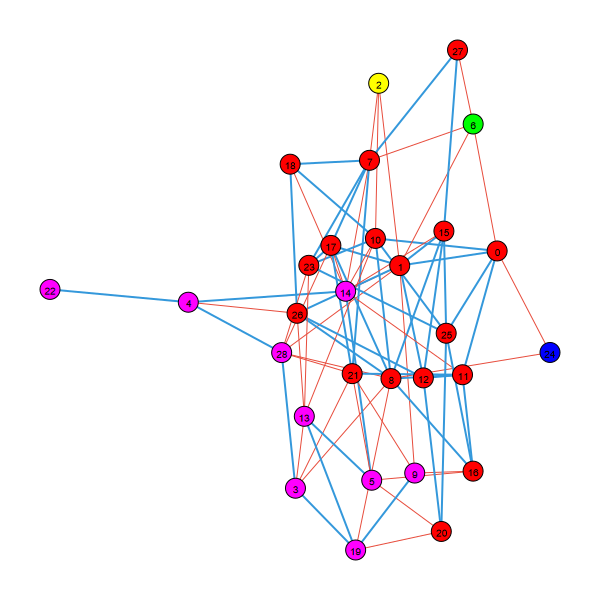
\includegraphics[width=0.6\textwidth]{imgs/clusters_network_d.png}
			\caption{Colored  graph of Network D by supernode assignments}
		\end{figure}
		\newpage
		\answer{
		\textbf{Network E}
		\textbf{Identified Super-nodes:} 2 factions\\
		\textbf{Result:} Unbalanced\\
		\textbf{Reason:} Internal contradiction: nodes 25 and 18 are friends but connected by a negative edge.
	
		\paragraph{Super-node Assignments}
		\begin{itemize}
			\item Super-node 0 (Size 25): $\{0,1,10,22,26,27,2,4,5,8,20,3,12,17\\\hfill
			,21,25,13,29,6,18,23,14,16,15,28\}$
			\item Super-node 1 (Size 5): $\{19,9,24,7,11\}$
		\end{itemize}
	}
		\begin{figure}[H]
			\centering
			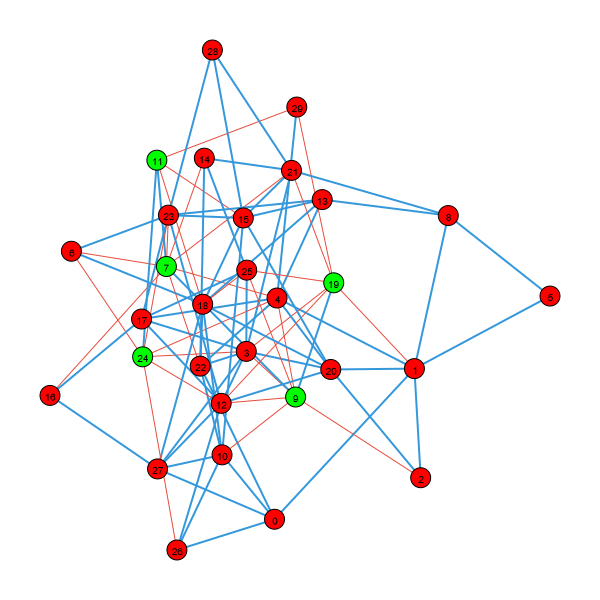
\includegraphics[width=0.6\textwidth]{imgs/clusters_network_e.png}
			\caption{Colored  graph of Network E by supernode assignments}
		\end{figure}
		\newpage
				\answer{
		\textbf{Network F}
		\textbf{Identified Super-nodes:} 3 factions\\
		\textbf{Result:} Strongly balanced\\
		\textbf{Reason:} The reduced graph is bipartite.
		
		\paragraph{Super-node Assignments}
		\begin{itemize}
			\item Super-node 0 (Size 27): $\{0,2,5,7,9,12,21,23,32,1,13,14,17, \\\hfill
			26,28,3,4,19,18,31,11,30,6,20,29,15,33\}$
			\item Super-node 1 (Size 1): $\{16\}$
			\item Super-node 2 (Size 6): $\{27,10,22,24,8,25\}$
		\end{itemize}
	}
		\begin{figure}[H]
			\centering
			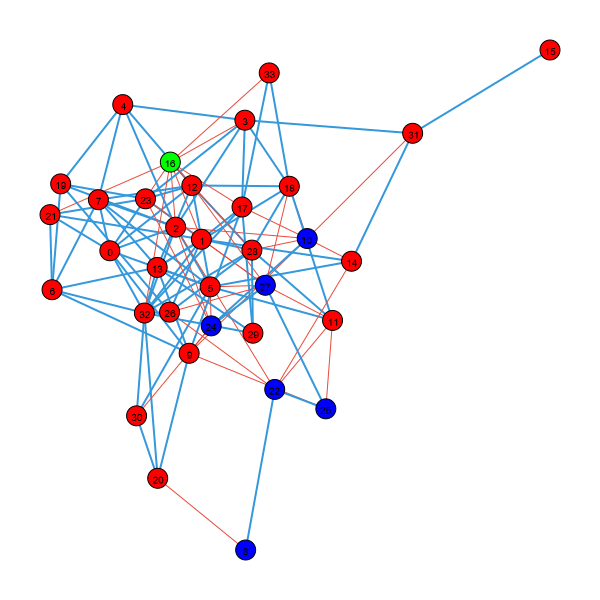
\includegraphics[width=0.6\textwidth]{imgs/clusters_network_f.png}
			\caption{Colored  graph of Network F by supernode assignments}
		\end{figure}
		\newpage
				\answer{
		\textbf{Network G}
		\textbf{Identified Super-nodes:} 3 factions\\
		\textbf{Result:} Unbalanced\\
		\textbf{Reason:} Internal contradiction: nodes 21 and 1 are friends but connected by a negative edge.
		
		\paragraph{Super-node Assignments}
		\begin{itemize}
			\item Super-node 0 (Size 19): $\{0,3,8,17,21,22,1,13,20,2,7,9,16,4,14,5,12,15,19\}$
			\item Super-node 1 (Size 3): $\{10,6,18\}$
			\item Super-node 2 (Size 1): $\{23\}$
		\end{itemize}
	}
		\begin{figure}[H]
			\centering
			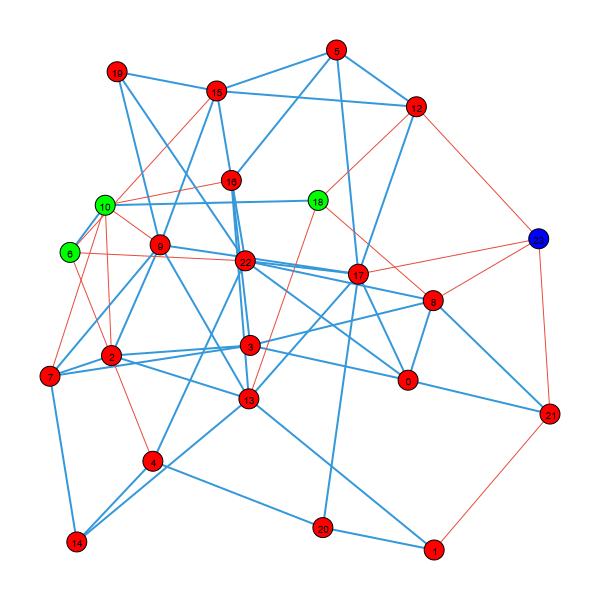
\includegraphics[width=0.6\textwidth]{imgs/clusters_network_g.png}
			\caption{Colored  graph of Network G by supernode assignments}
		\end{figure}
		\newpage
				\answer{
		\textbf{Network H}
		\textbf{Identified Super-nodes:} 5 factions\\
		\textbf{Result:} Strongly balanced\\
		\textbf{Reason:} The reduced graph is bipartite.
		
		\paragraph{Super-node Assignments}
		\begin{itemize}
			\item Super-node 0 (Size 25): $\{0,1,13,21,22,8,19,24,25,2,23,3,11,17,\\\hfill
			4,12,20,28,18,16,10,27,29,14,15\}$
			\item Super-node 1 (Size 2): $\{26,7\}$
			\item Super-node 2 (Size 1): $\{6\}$
			\item Super-node 3 (Size 1): $\{9\}$
			\item Super-node 4 (Size 1): $\{5\}$
		\end{itemize}
	}
		\begin{figure}[H]
			\centering
			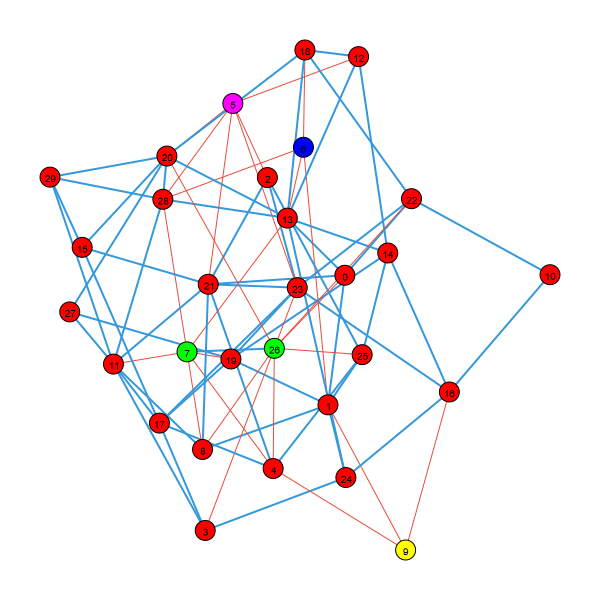
\includegraphics[width=0.6\textwidth]{imgs/clusters_network_h.png}
			\caption{Colored  graph of Network H by supernode assignments}
		\end{figure}
		\newpage
	\end{subquestion}
	\begin{subquestion}{Clusterability}
		\answer{
		We used the same method as the last question but here we didn't enforce bipartitness and allowed weakly balanced networks
		}
		\answer{
		\textbf{Network A}
		\textbf{Identified Super-nodes:} 3 factions \\
		\textbf{Result:} Strongly balanced\\
		\textbf{Reason:} The reduced graph is bipartite. Since every strongly balanced graph is also weakly balanced, this network satisfies the conditions for weak structural balance. Moreover, because the reduced graph admits a bipartition into two opposing groups, clusters 2 and 0 can be merged. By the definition of strong structural balance for incomplete networks, this results in a strongly balanced network.

		
		\paragraph{Super-node Assignments}
		\begin{itemize}
			\item Super-node 0 (Size 5): $\{4,7,12,2,0\}$
			\item Super-node 1 (Size 5): $\{1,3,13,11,10\}$
			\item Super-node 2 (Size 4): $\{9,5,8,6\}$
		\end{itemize}
	}
		\begin{figure}[H]
			\centering
			
\includegraphics[width=0.6\textwidth]{imgs/q4_partc_images/clusters_network_a.png}
			\caption{Colored graph of Network A by cluster assignment}
		\end{figure}
		\newpage
		\answer{
		\textbf{Network B}
		\textbf{Identified Super-nodes:} 4 factions\\
		\textbf{Result:} Weakly balanced\\
		\textbf{Reason:} No inner-cluster negative edges are present, but the reduced graph is not bipartite.
		
		\paragraph{Super-node Assignments}
		\begin{itemize}
			\item Super-node 0 (Size 5): $\{14,10,9,0,8\}$
			\item Super-node 1 (Size 5): $\{5,15,12,18,2\}$
			\item Super-node 2 (Size 5): $\{7,6,13,17,3\}$
			\item Super-node 3 (Size 5): $\{19,1,11,16,4\}$
		\end{itemize}
	}
		\begin{figure}[H]
			\centering
			
\includegraphics[width=0.6\textwidth]{imgs/q4_partc_images/clusters_network_b.png}
			\caption{Colored graph of Network B by cluster assignment}
		\end{figure}
		\newpage
		\answer{		
		\textbf{Network C}
		\textbf{Identified Super-nodes:} 4 factions\\
		\textbf{Result:} Weakly balanced\\
		\textbf{Reason:} No inner-cluster negative edges are present, but the reduced graph is not bipartite.
		
		\paragraph{Super-node Assignments}
		\begin{itemize}
			\item Super-node 0 (Size 8): $\{10,13,29,19,7,21,11,16\}$
			\item Super-node 1 (Size 8): $\{1,25,14,15,20,17,24,26\}$
			\item Super-node 2 (Size 7): $\{5,18,8,27,3,28,22\}$
			\item Super-node 3 (Size 7): $\{4,2,9,12,6,23,0\}$
		\end{itemize}
	}
		\begin{figure}[H]
			\centering
			
\includegraphics[width=0.6\textwidth]{imgs/q4_partc_images/clusters_network_c.png}
			\caption{Colored graph of Network C by cluster assignment}
		\end{figure}
		\newpage
		\answer{
		\textbf{Network D}
		\textbf{Identified Super-nodes:} 6 factions\\
		\textbf{Result:} Weakly balanced\\
		\textbf{Reason:} No inner-cluster negative edges are present, but the reduced graph is not bipartite.
		
		\paragraph{Super-node Assignments}
		\begin{itemize}
			\item Super-node 0 (Size 7): $\{33,4,7,12,14,39,0\}$
			\item Super-node 1 (Size 7): $\{34,1,31,35,6,19,29\}$
			\item Super-node 2 (Size 7): $\{16,17,21,2,36,15,8\}$
			\item Super-node 3 (Size 7): $\{24,27,37,20,28,9,5\}$
			\item Super-node 4 (Size 6): $\{32,38,3,26,11,13\}$
			\item Super-node 5 (Size 6): $\{10,18,23,30,22,25\}$
		\end{itemize}
	}
		\begin{figure}[H]
			\centering
			
\includegraphics[width=0.6\textwidth]{imgs/q4_partc_images/clusters_network_d.png}
			\caption{Colored graph of Network D by cluster assignment}
		\end{figure}
		\newpage
		\answer{
		\textbf{Network E}
		\textbf{Identified Super-nodes:} 8 factions\\
		\textbf{Result:} Weakly balanced\\
		\textbf{Reason:} No inner-cluster negative edges are present, but the reduced graph is not bipartite.
		
		\paragraph{Super-node Assignments}
		\begin{itemize}
			\item Super-node 0 (Size 8): $\{48,26,9,12,18,0,54,46\}$
			\item Super-node 1 (Size 8): $\{16,50,11,58,47,2,27,23\}$
			\item Super-node 2 (Size 8): $\{24,14,21,5,6,32,56,43\}$
			\item Super-node 3 (Size 8): $\{22,42,25,29,52,49,34,31\}$
			\item Super-node 4 (Size 7): $\{19,53,1,8,4,7,13\}$
			\item Super-node 5 (Size 7): $\{35,41,36,3,55,30,10\}$
			\item Super-node 6 (Size 7): $\{28,17,37,39,44,59,33\}$
			\item Super-node 7 (Size 7): $\{57,15,38,45,20,40,51\}$
		\end{itemize}
	}
		\begin{figure}[H]
			\centering
			
\includegraphics[width=0.6\textwidth]{imgs/q4_partc_images/clusters_network_e.png}
			\caption{Colored graph of Network E by cluster assignment}
		\end{figure}
		\newpage
	\end{subquestion}
	\begin{subquestion}{Line Index:}
		\begin{enumerate}
			\item Random clustering:
			\answer{
				The functions \textbf{assign\_random} and \textbf{calculate\_line\_index} perform the random cluster assignment and the line index calculation, respectively. The function \textbf{find\_edge\_between\_clusters} iterates over all combinations of vertices from different clusters and identifies positive and negative edges between them, which aids in the computation of the line index.
			}
			
			\item Heuristic:
			\answer{
				The function \textbf{fix\_clusters} implements a local search optimization procedure to refine social cluster assignments by minimizing structural tension. It iteratively evaluates each node to determine whether moving it to a different cluster would reduce the total cost function, namely the line index. The algorithm continues looping through all nodes until a local optimum is reached, meaning that no single node movement can further reduce the cost. This process ensures that each individual is assigned to the faction in which they experience the fewest social contradictions.
				
				\paragraph{Algorithm Results}
				a sample of the performance of the clustering algorithm is summarized below.
				
				\begin{itemize}
					\item \textbf{Initial random assignment:}
					\begin{itemize}
						\item Positive edges between clusters ($P$): 66
						\item Negative edges within clusters ($N$): 13
						\item Initial line index: 39.5
					\end{itemize}
					
					\item \textbf{After cluster optimization (local search):}
					\begin{itemize}
						\item Positive edges between clusters ($P$): 0
						\item Negative edges within clusters ($N$): 0
						\item Final line index: 0.0
					\end{itemize}
				\end{itemize}
				
				The algorithm achieves a total reduction in frustration of $39.5$, indicating that the final clustering eliminates all structural inconsistencies and attains a fully balanced configuration.
				
			}
		\end{enumerate}
		
	\end{subquestion}
\end{question}